In this section we describe the results along with the specific details of the algorithms used for each problem. We solve every problem with both penalty and augmented Lagrangian methods.
\begin{itemize}
    \item \textbf{Architecture}: We use two different types of architecture in our experiments, see appendix~\ref{ssec-arch--var-ml} for a description of these types and refer to table~\ref{tab:network--var-ml} for details of $\mathcal A, \mathcal B$ used in the experiments. We use the same architecture to represent the approximate solutions of penalty and augmented Lagrangian algorithms.
    \item \textbf{Stopping criteria}: Although sophisticated stopping criteria such as the norm of the gradient of the objective function in the subproblem falling below a pre-selected threshold, can be used for algorithms~\ref{algo:dl-penalty--var-ml}, \ref{algo:dl-al-finite--var-ml}, \ref{algo:dl-al-infinite--var-ml}, here we stop the loops after a pre-selected number of iterations is reached.
    \item \textbf{Number of gradient descent steps}: We denote this number of iterations with $P$ for the outer loops in algorithms~\ref{algo:dl-penalty--var-ml}, \ref{algo:dl-al-finite--var-ml}, \ref{algo:dl-al-infinite--var-ml}, $Q$ for the inner loops in algorithms~\ref{algo:dl-penalty--var-ml}, \ref{algo:dl-al-finite--var-ml} and $Q^A,Q^B$ for the first and second inner loops in the algorithm~\ref{algo:dl-al-infinite--var-ml} respectively. We define $E$ to be the total number of gradient descent steps used. Therefore, $E=PQ$ for algorithms~\ref{algo:dl-penalty--var-ml} and \ref{algo:dl-al-finite--var-ml} and $E=P(Q^A+Q^B)$ for algorithm~\ref{algo:dl-al-infinite--var-ml}. For each problem we use the same total gradient descent steps $E$ for both the penalty and the augmented Lagrangian algorithms. To facilitate this, when $W$ is finite dimensional we use the same $Q$ for algorithms~\ref{algo:dl-penalty--var-ml} and \ref{algo:dl-al-finite--var-ml} and when $W$ is infinite dimensional we set $Q^A=Q^B=Q/2$. We use the popular Adam optimizer \cite{kingma2014adam} to perform the gradient descent steps.
    \item\textbf{Learning rate}: We use an initially oscillating and finally decaying learning rate $\delta$ that depends on 7 distinct hyperparameters. The oscillatory nature of $\delta$ as seen in figure~\ref{fig:learning-rate--var-ml}, is employed to essentially rejuvenate the previously decaying learning rate every time we start  an inner loop in the algorithms. For details of this learning rate $\delta$, see appendix~\ref{ssec-rate--var-ml}. 
\begin{figure}[!ht]
    \centering
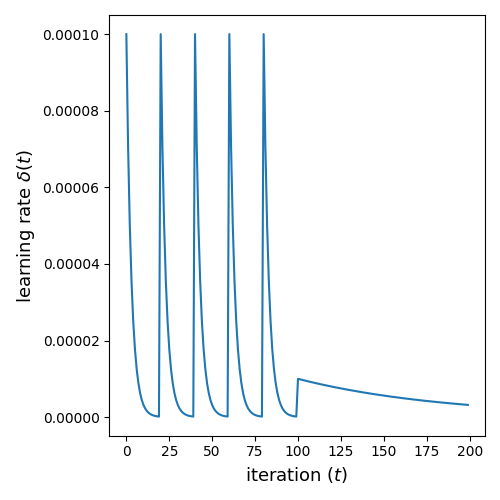
\includegraphics[scale=0.5
]{var-ml/plots/var-plots-learning-rate.png}
    \caption{Example behavior of the oscillating learning rate $\delta$}
    \label{fig:learning-rate--var-ml}
\end{figure}
While using algorithms~\ref{algo:dl-penalty--var-ml} and \ref{algo:dl-al-finite--var-ml} we set,
\begin{align}
    \delta_{k, j}=\delta((k-1)Q+j)
\end{align}
and while using algorithm~\ref{algo:dl-al-infinite--var-ml} we use,
\begin{align}
    \delta_{k, j}^A = \delta((k-1)Q^A+j)\\
    \delta_{k, j}^B = \delta((k-1)Q^B+j)
\end{align}
\item\textbf{The penalty factors}: We use a stopped geometric sequence as our $\mu_k$,
\begin{align}
    \mu_k=\min\{\mu_1r^{k-1},\mu_{\max}\}\label{eq:mu--var-ml}
\end{align}
The exact values of $\mu_1,\mu_{\max}, r$ for various problems can be found in table~\ref{tab:mu--var-ml}.
\item \textbf{Computation of functionals}: To compute the functional $f$ and when $W$ is infinite dimensional, the functional $|\cdot|_W$, we use either Gauss-Legendre quadrature (in 1 or 2 dimensions) or a Monte Carlo estimate (in 3 dimensions).
\item\textbf{Errors}: We evaluate our algorithms using three different kinds of errors produced.
If $\hat u$ is the solution produced by an algorithm and $u^{\rm true}$ is the true solution the problem we define the absolute error to be an weighted $L^2$-norm  of $\hat u-u^{\rm true}$,
\begin{align}
{\rm absolute\;error}=\sqrt{\frac{\int_{\Omega}(\hat u-u^{\rm true})^2\,dV}{\int_{\Omega}\,dV}}
\end{align}
where $dV$ denotes a volume element in $\Omega$. We define the relative objective error to be the relative error in the value of the objective function, 
\begin{align}
{\rm relative\; objective\; error}=\left|\frac{f(\hat u)-f(u^{\rm true})}{f(u^{\rm true})}\right|\label{eq:rel-err--var-ml}
\end{align}
\end{itemize}
And lastly, we define the constraint error to be how closely $\hat u$ satisfies the constraint,
\begin{align}
    {\rm constraint\; error}= |g(\hat u)|_W
\end{align}
With these definitions we are now ready to present the results.     

\subsection{The minimal surface problem}
Figure~\ref{fig:helicoid-surface--var-ml} shows the true and approximate solutions to the minimal surface problem in Cartesian coordinates. The true solution for this problem is a helicoid. 
\begin{figure}[!ht]
    \centering
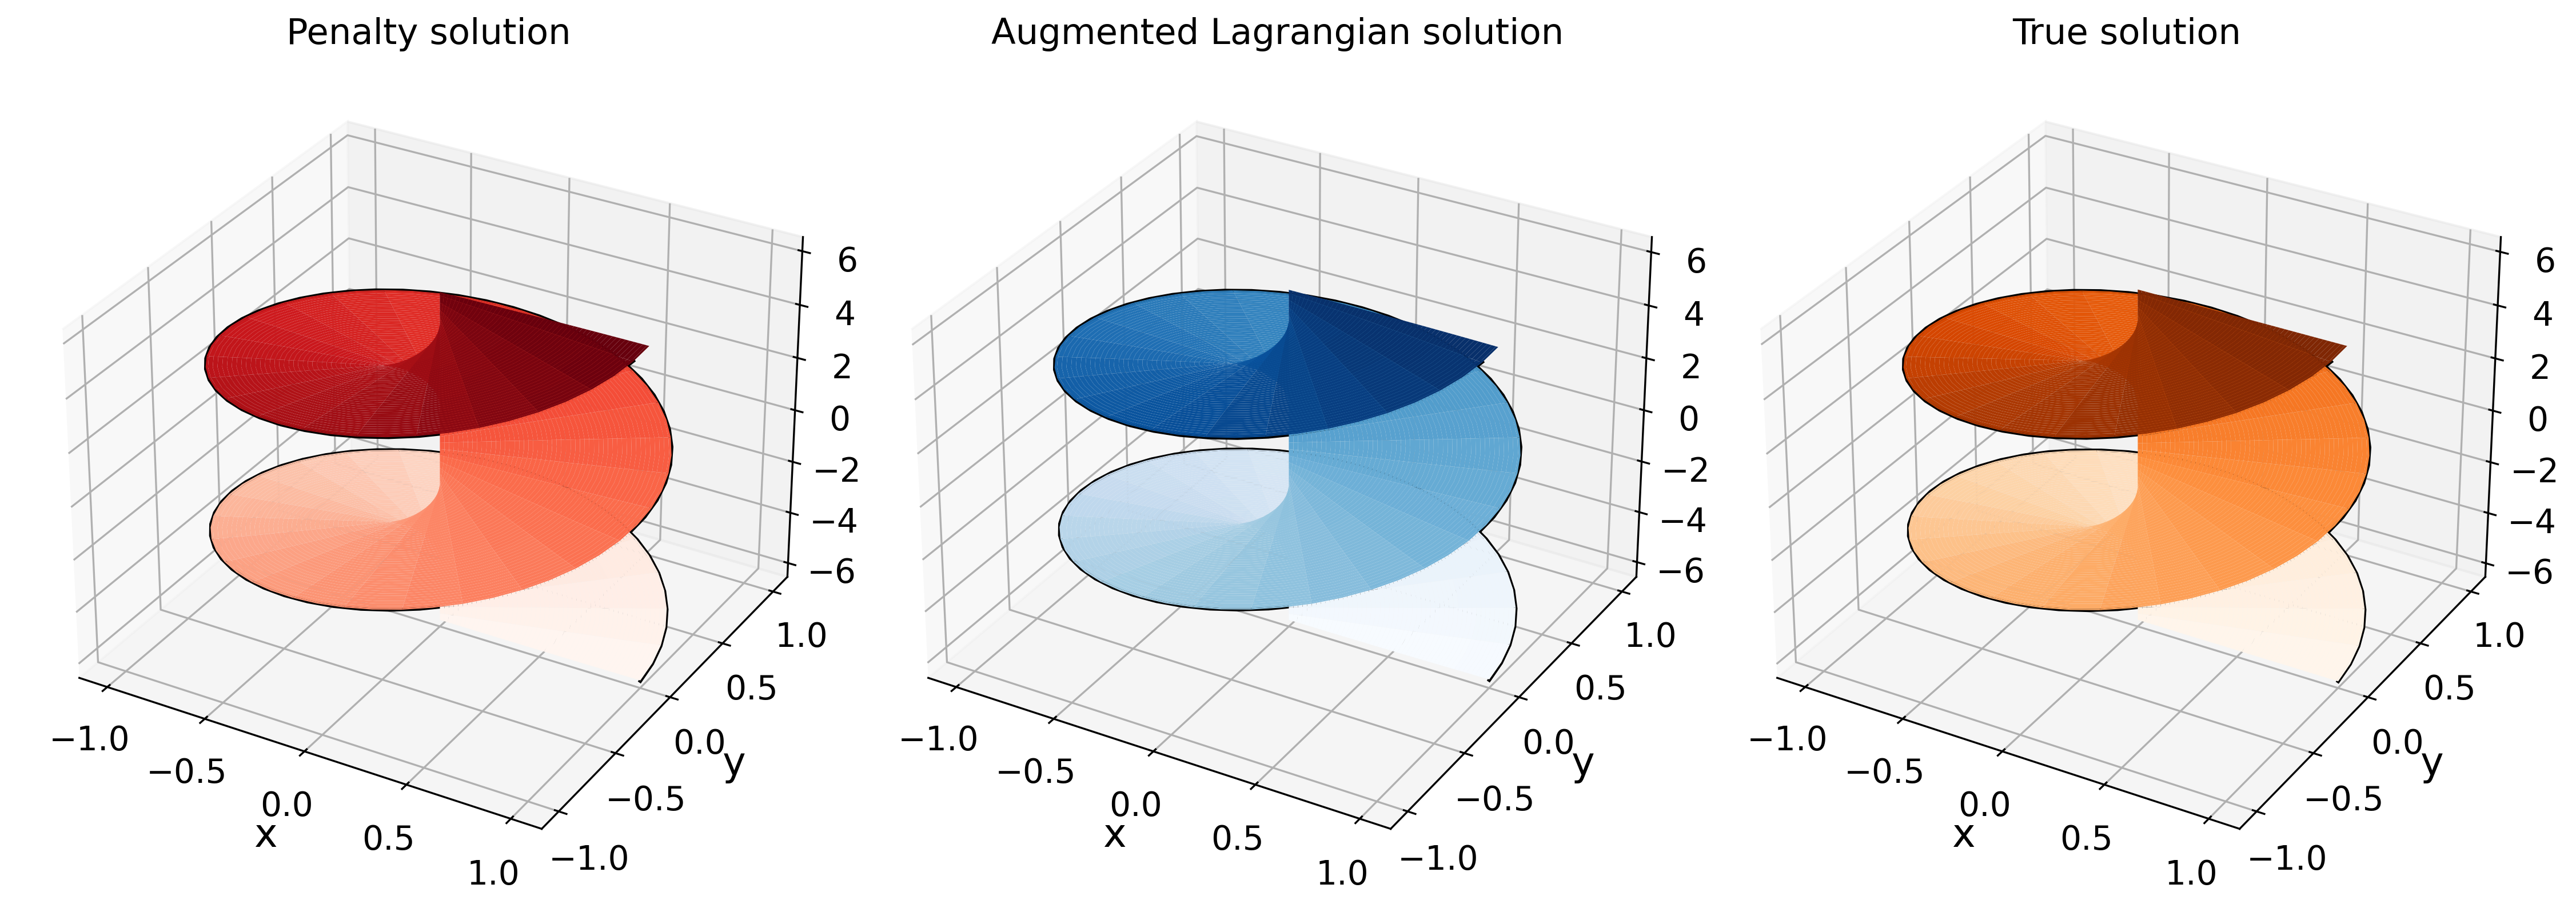
\includegraphics[scale=0.4]{var-ml/plots/var-plots-helicoid-surface.png}
    \caption{Solutions to the minimal surface problem}
    \label{fig:helicoid-surface--var-ml}
\end{figure}
% For this problem we define the absolute error to be,
% \begin{align}
% {\rm absolute\;error}=\sqrt{\frac{\int_{-2\pi}^{2\pi}\int_0^1(\hat u-u^{\rm true})^2r\,dr\,d\theta}{\int_{-2\pi}^{2\pi}\int_0^1r\,dr\,d\theta}}   
% \end{align}
We use $E=20000$ total gradient steps and $P=1000$ subproblems for this problem. This setup implies to calculate solutions to the subproblems, we use $Q=20$ gradient descent steps for the penalty algorithm (${\rm P}^\infty$) and $Q^A=Q^B=10$ gradient steps for the augmented Lagrangian algorithm (${\rm AL}^\infty_\infty$). Figure~\ref{fig:helicoid-error--var-ml} shows various errors as functions of gradient descent steps for this problem. In terms of algorithms~\ref{algo:dl-penalty--var-ml}, \ref{algo:dl-al-finite--var-ml}, \ref{algo:dl-al-infinite--var-ml}, iteration in figure~\ref{fig:helicoid-error--var-ml} can be understood as $(k-1)E/P+j$. The errors and run times have been plotted every 100 steps.
\begin{figure}[!ht]
    \centering
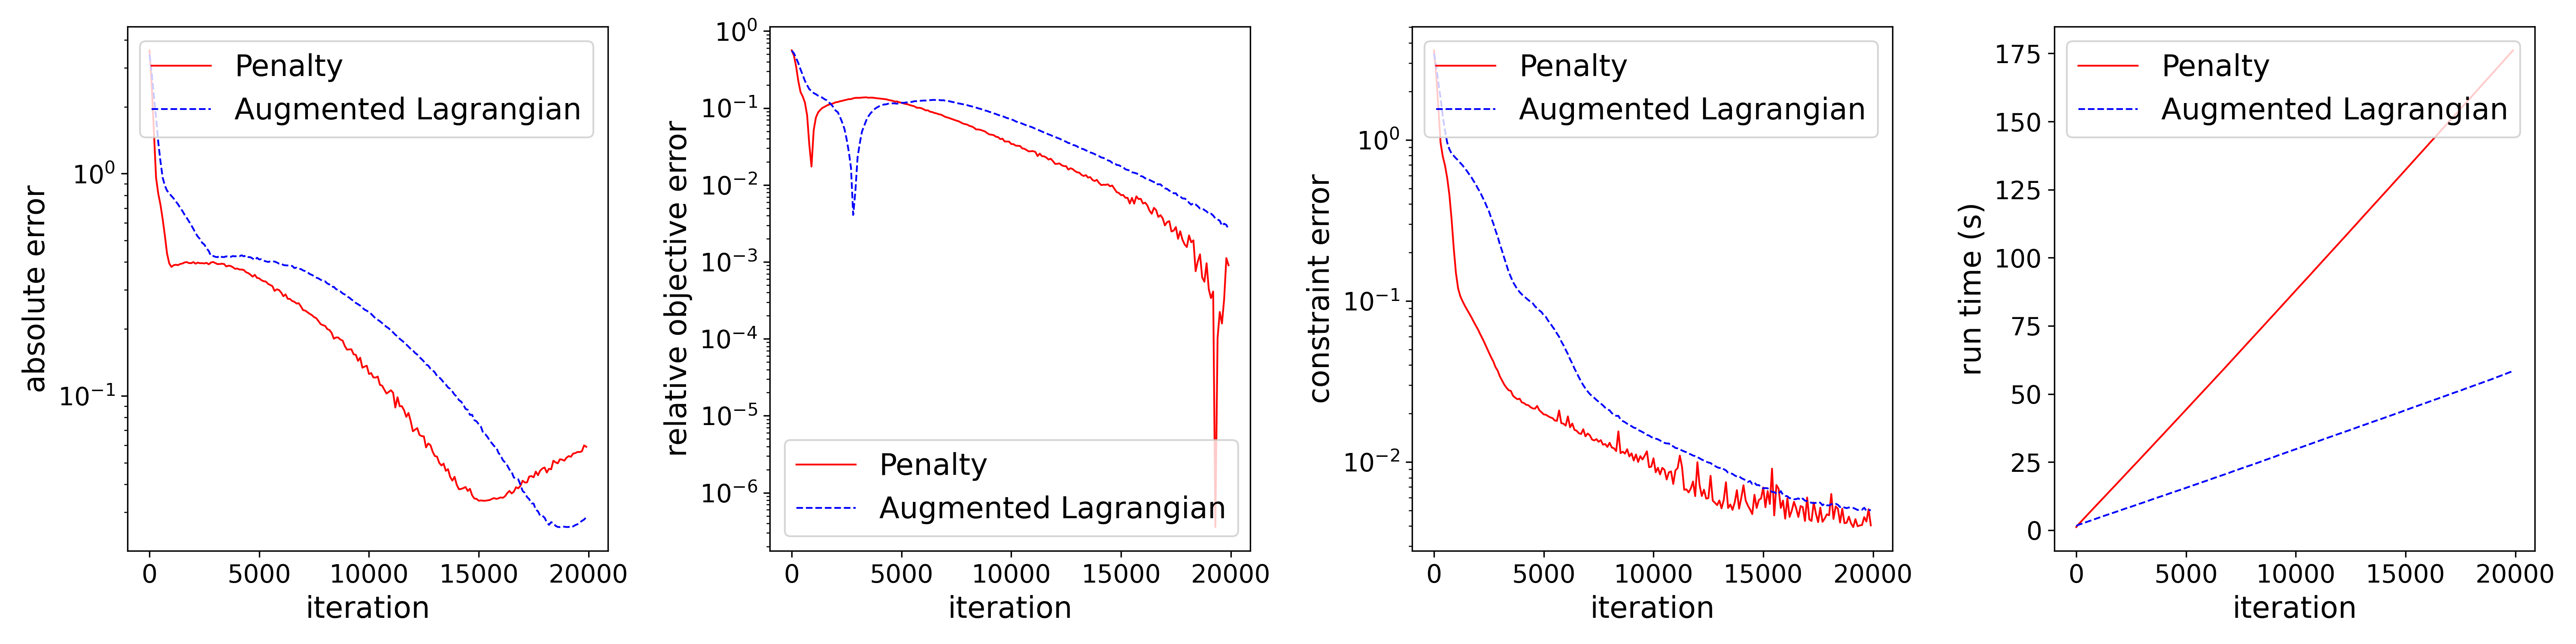
\includegraphics[scale=0.32]{var-ml/plots/var-plots-helicoid-error.png}
    \caption{Errors and run times for the minimal surface problem as functions of gradient descent steps. The errors have been plotted in a semilog fashion. All quantities have been plotted every 100 steps.}
    \label{fig:helicoid-error--var-ml}
\end{figure}
Both methods are able to produce good approximations but the penalty method fluctuates more during training compared to its counterpart for this problem. Looking at table~\ref{tab:network--var-ml} we see that sizes of the networks representing the solution and the Lagrange multiplier $a, b$ are close to each other. But solving the problem \eqref{eq:xi-update--var-ml} is computationally much cheaper than solving the problem \eqref{eq:seq-uncon-al-net--var-ml}. This is a typical scenario and is reflected in the run times of the algorithms in figure~\ref{fig:helicoid-error--var-ml} where the augmented Lagrangian is $3.016$ times faster than its counterpart.

\subsection{Geodesics on a surface}
Figure~\ref{fig:geo--var-ml} shows the approximate solutions to the geodesic problem. The true solution to this problem is the arc between the given points that lies on the great circle connecting them.
\begin{figure}[!ht]
    \centering
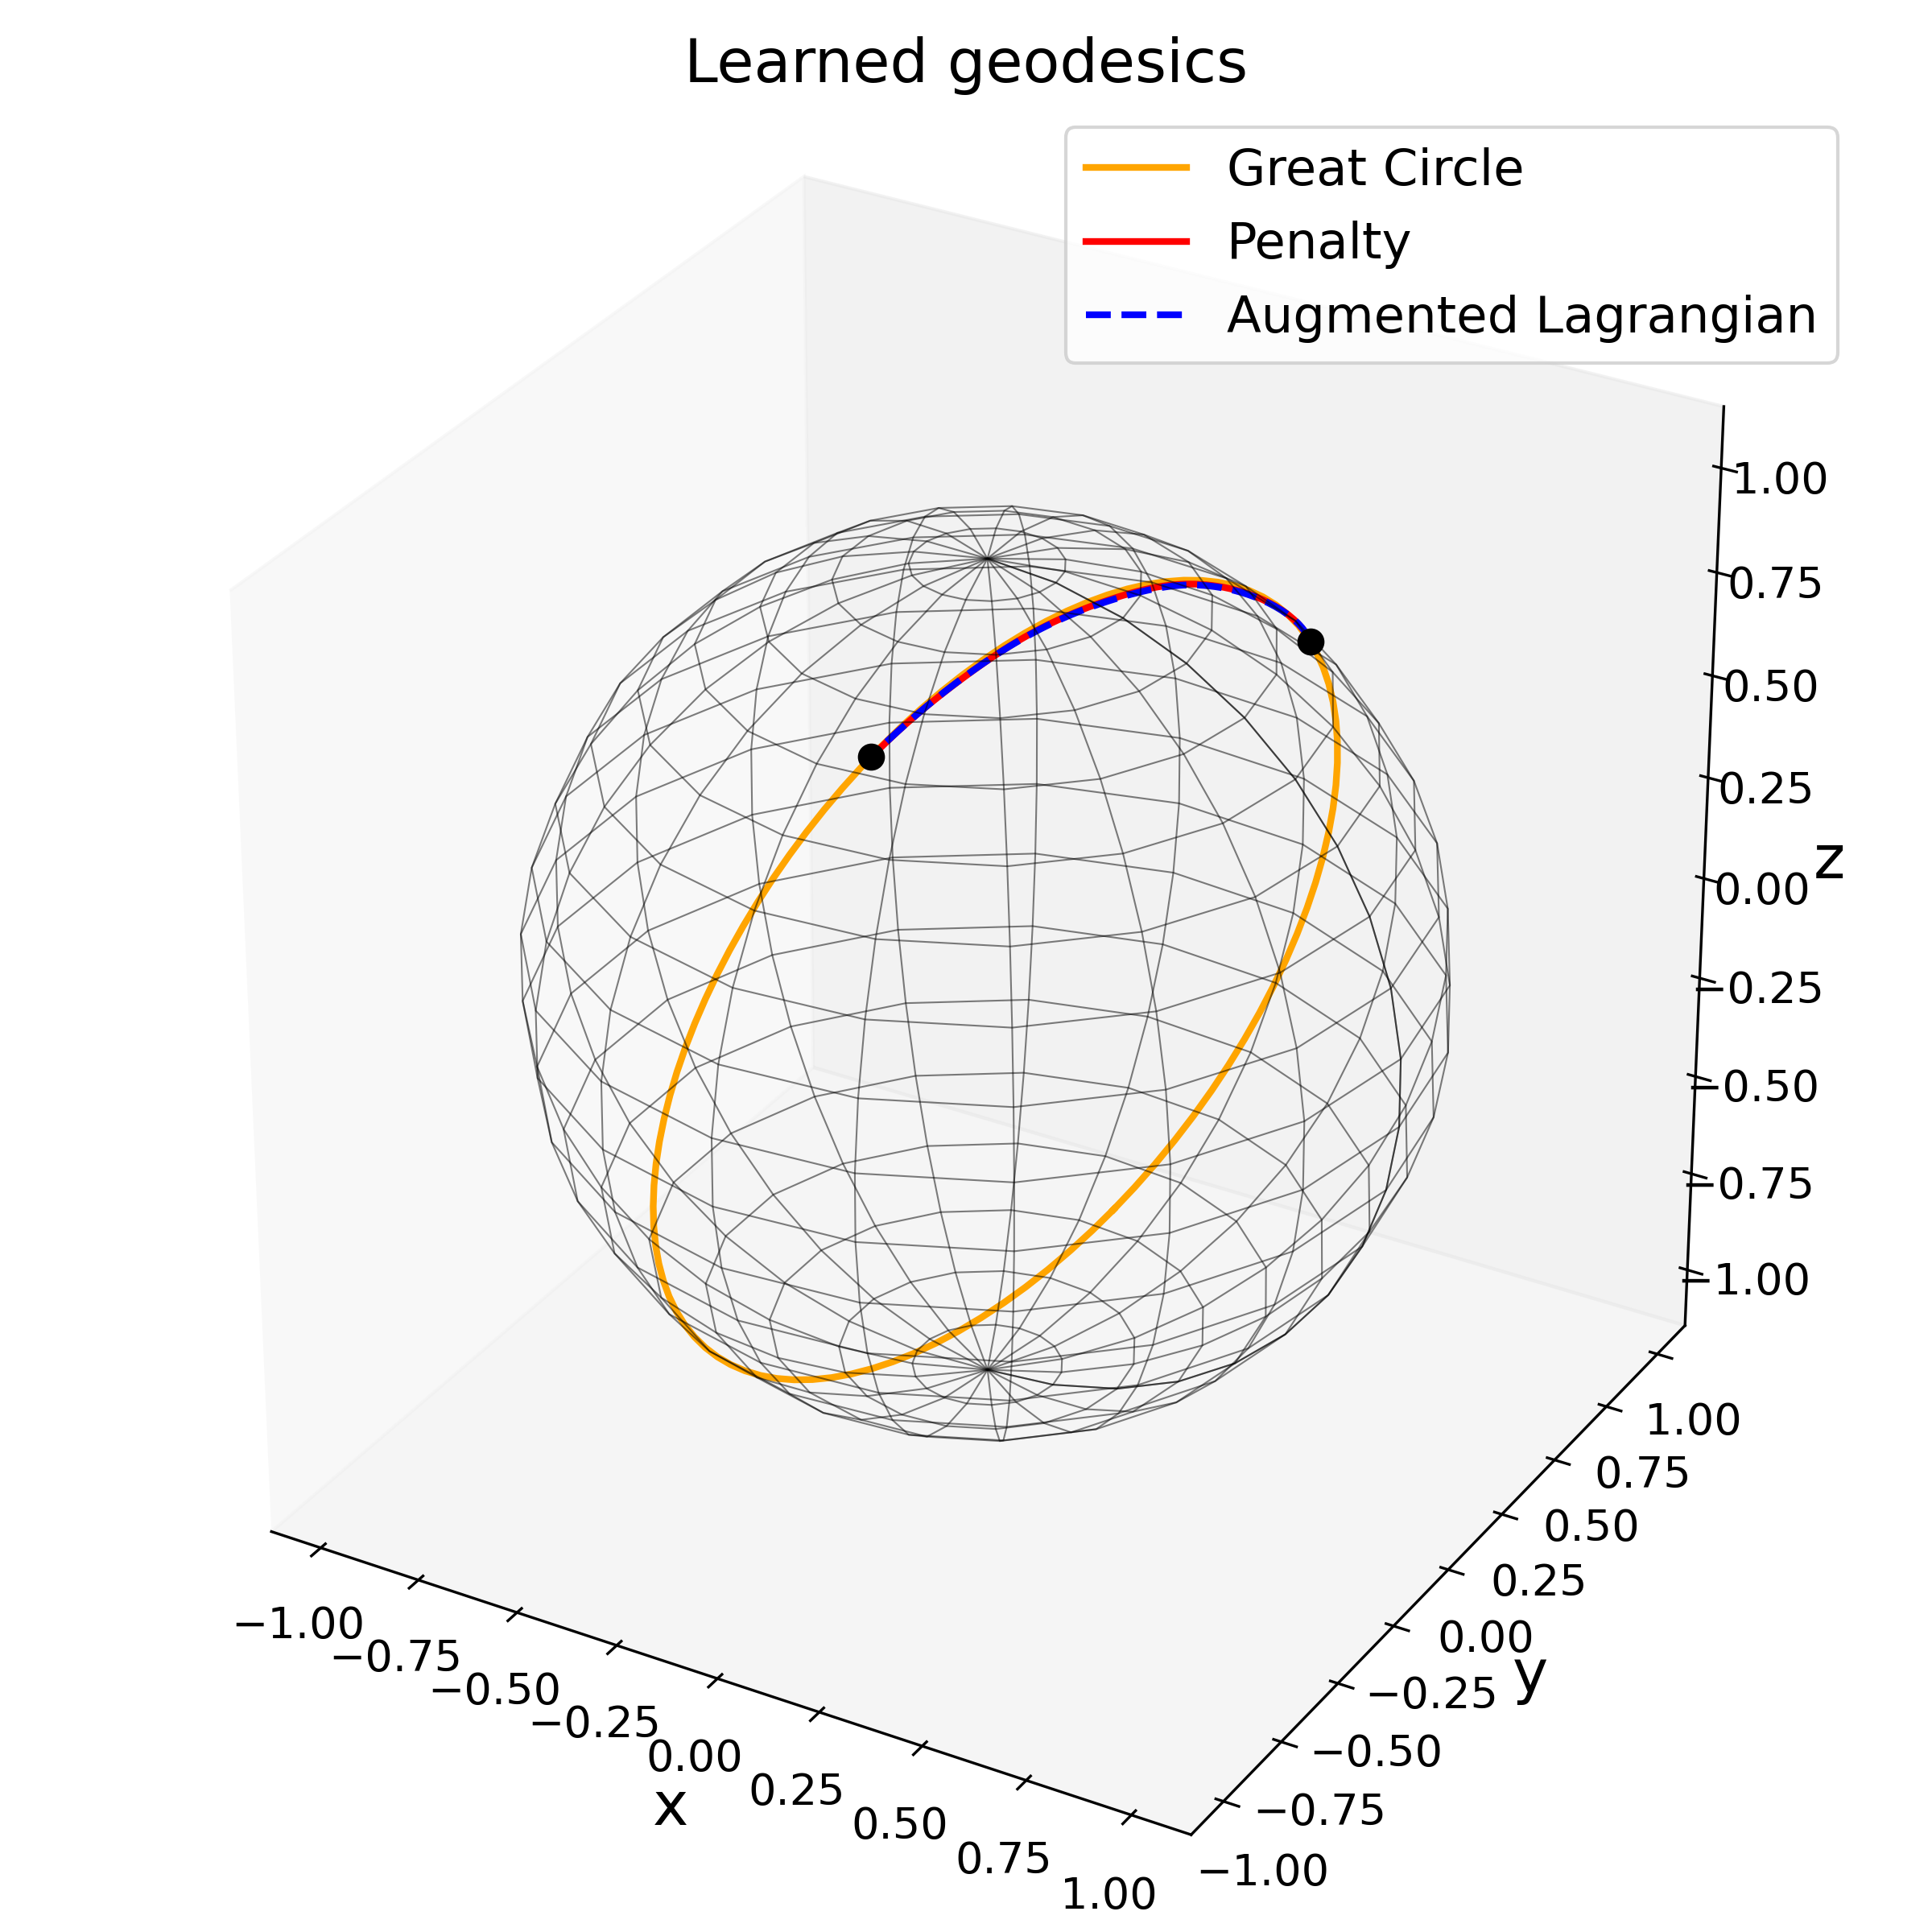
\includegraphics[scale=0.4]{var-ml/plots/var-plots-sphere-geodesic.png}
    \caption{Solutions to the geodesic problem. The distance between the black dots is being minimized.}
    \label{fig:geo--var-ml}
\end{figure}
% For this problem we define the absolute error as,
% \begin{align}
% {\rm absolute\;error}=\sqrt{\frac{\int_{\theta_0}^{\theta_1}(\hat u-u^{\rm true})^2\,d\theta}{\int_{\theta_0}^{\theta_1}\,d\theta}} 
% \end{align}
We use $E=50000$ and $P=2500$ for this problem which implies the number of gradient steps used to solve subproblems for the both the penalty (${\rm P}^\infty$) and the augmented Lagrangian (${\rm AL}^\infty_{\rm F}$) algorithms is $Q=20$. Figure~\ref{fig:geo-error--var-ml} shows the errors and run times for this problem as a function of gradient steps.
\begin{figure}[!ht]
    \centering
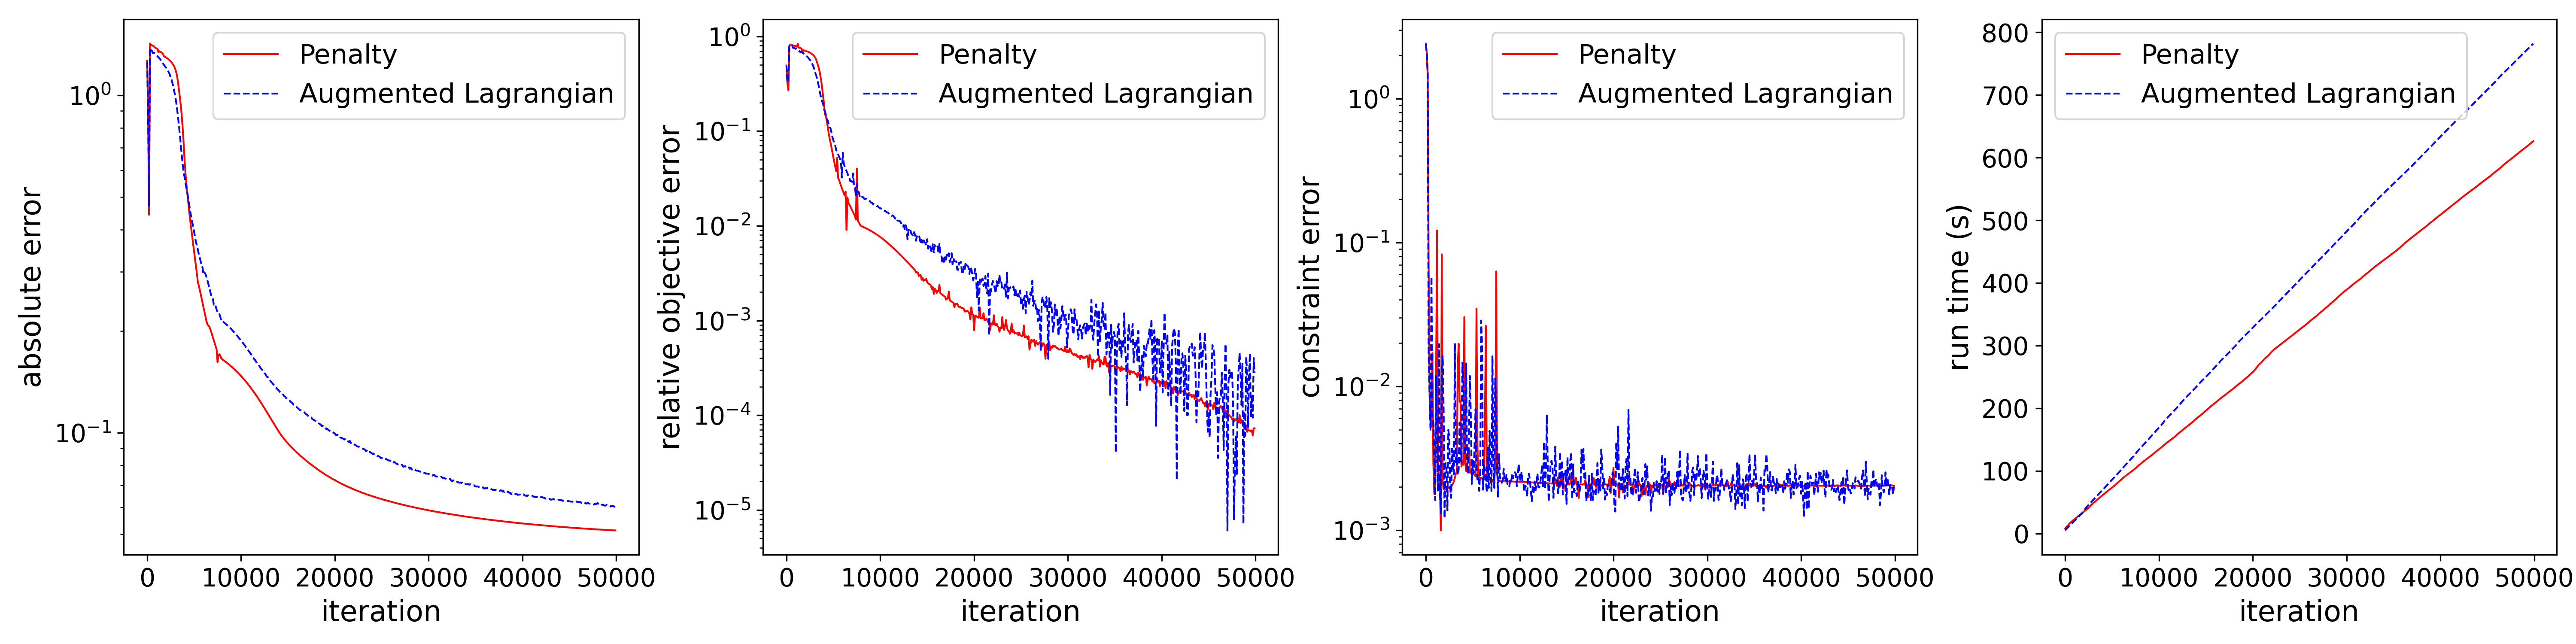
\includegraphics[scale=0.32]{var-ml/plots/var-plots-sphere-geodesic-error.png}
    \caption{Errors and run times for the geodesic problem as functions of gradient descent steps. The errors have been plotted in a semilog fashion. All quantities have been plotted every 100 steps.}
    \label{fig:geo-error--var-ml}
\end{figure}
 Although the absolute error decreases without significant fluctuations, ${\rm AL}^\infty_{\rm F}$ shows considerably more fluctuations in other errors compared to its counterpart during training. Since \eqref{eq:seq-uncon-al-net--var-ml} is computationally more expensive to solve than \eqref{eq:seq-uncon-net--var-ml} and we use the same number of gradient descent steps to solve both of them, the augmented Lagrangian algorithm is slower in this case as seen in figure~\ref{fig:geo-error--var-ml}.

In figure~\ref{fig:geo--var-ml} the points on the sphere are chosen to be nonantipodal, leading to a unique solution to the geodesic problem. In case these points are antipodal there are infinitely many great circles that connect them, leading to infinitely many solutions. The solution set in this degenerate case is homeomorphic to a connected 1D manifold. Figure~\ref{fig:geo-ap--var-ml} shows the geodesics learned with the penalty method for such a degenerate problem. As can be seen, the solution produced by the penalty algorithm (${\rm P}^\infty$) quite surprisingly does not hop from one great circle to another but rather stays on a single great circle with more and more gradient descent steps. Even though the true minima of the original problem lie on a connected manifold, the discretized version of the problem where we look for $\eta\in\mathbb R^a$, might have a different distribution of minima, where possibly each minimum can be separated from any other minimum by open sets.
\begin{figure}[!ht]
    \centering
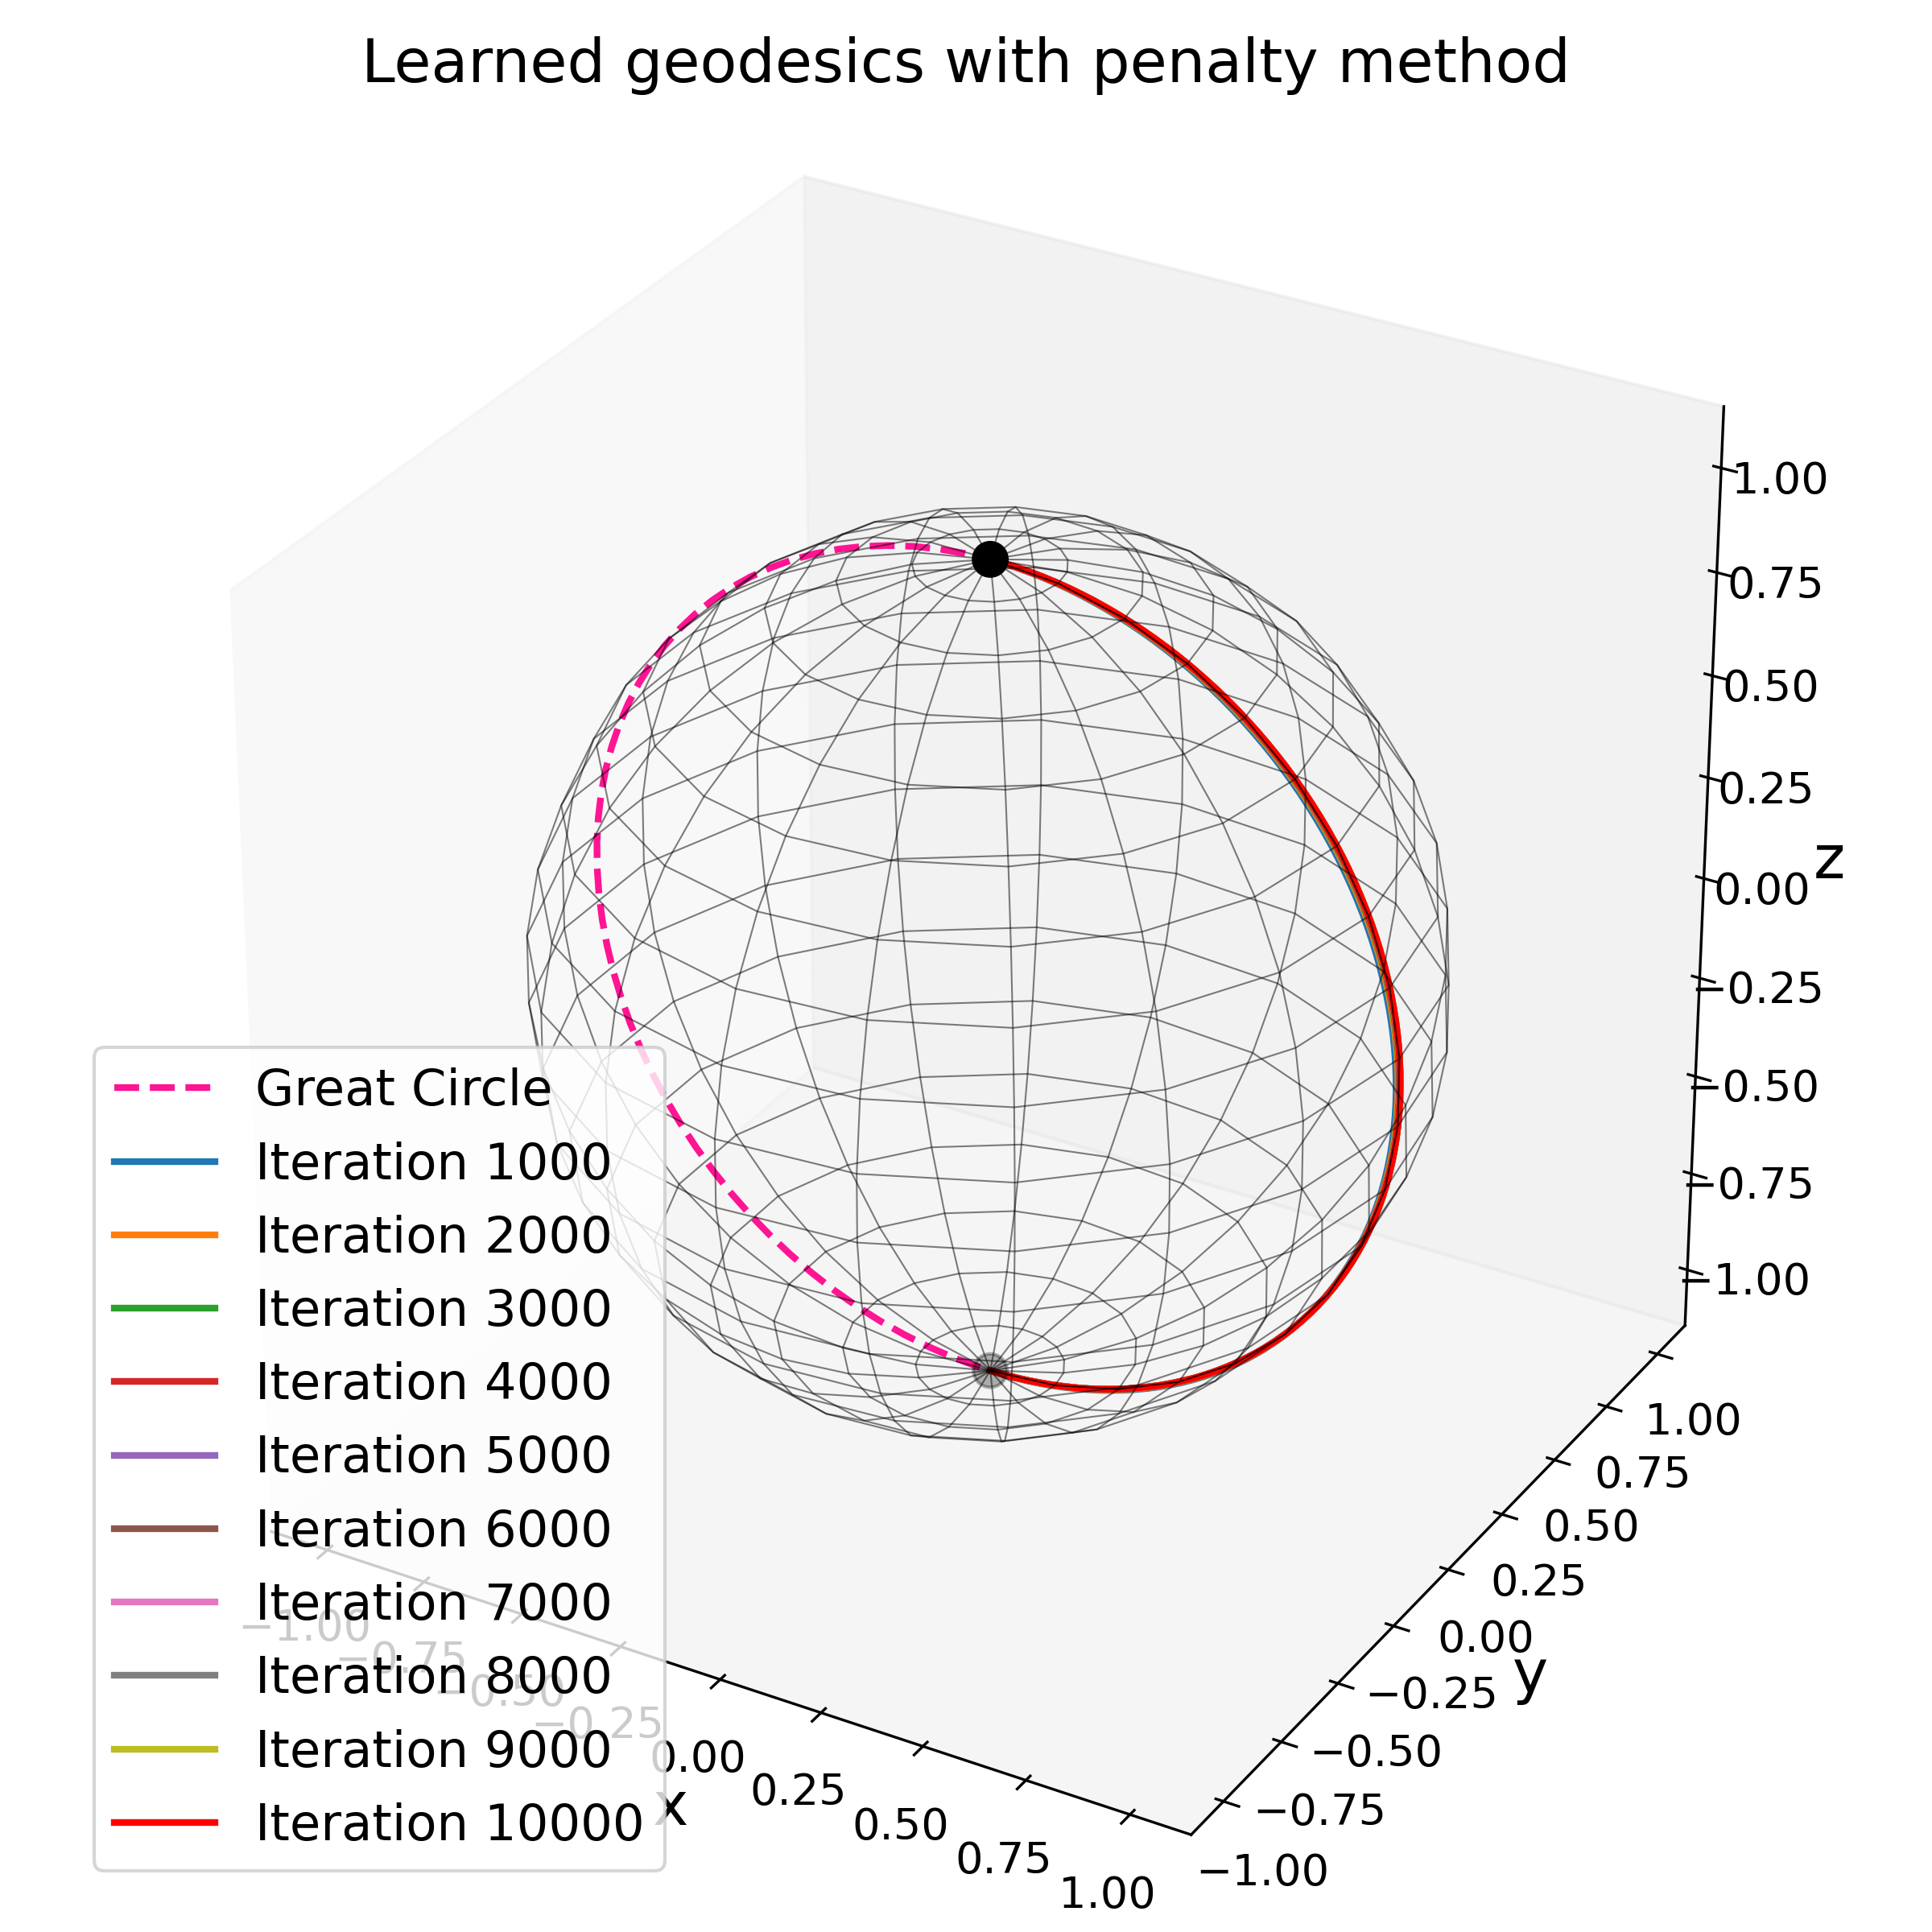
\includegraphics[scale=0.4]{var-ml/plots/var-plots-sphere-geodesic-antipodal.png}
    \caption{Solutions to the geodesic problem when the points (black dots) are antipodal}
    \label{fig:geo-ap--var-ml}
\end{figure}
\subsection{Grad-Shafranov equation}
Figure~\ref{fig:gs-surface--var-ml} shows the approximate and true solutions for the Grad-Shafranov equation.
\begin{figure}[!ht]
    \centering
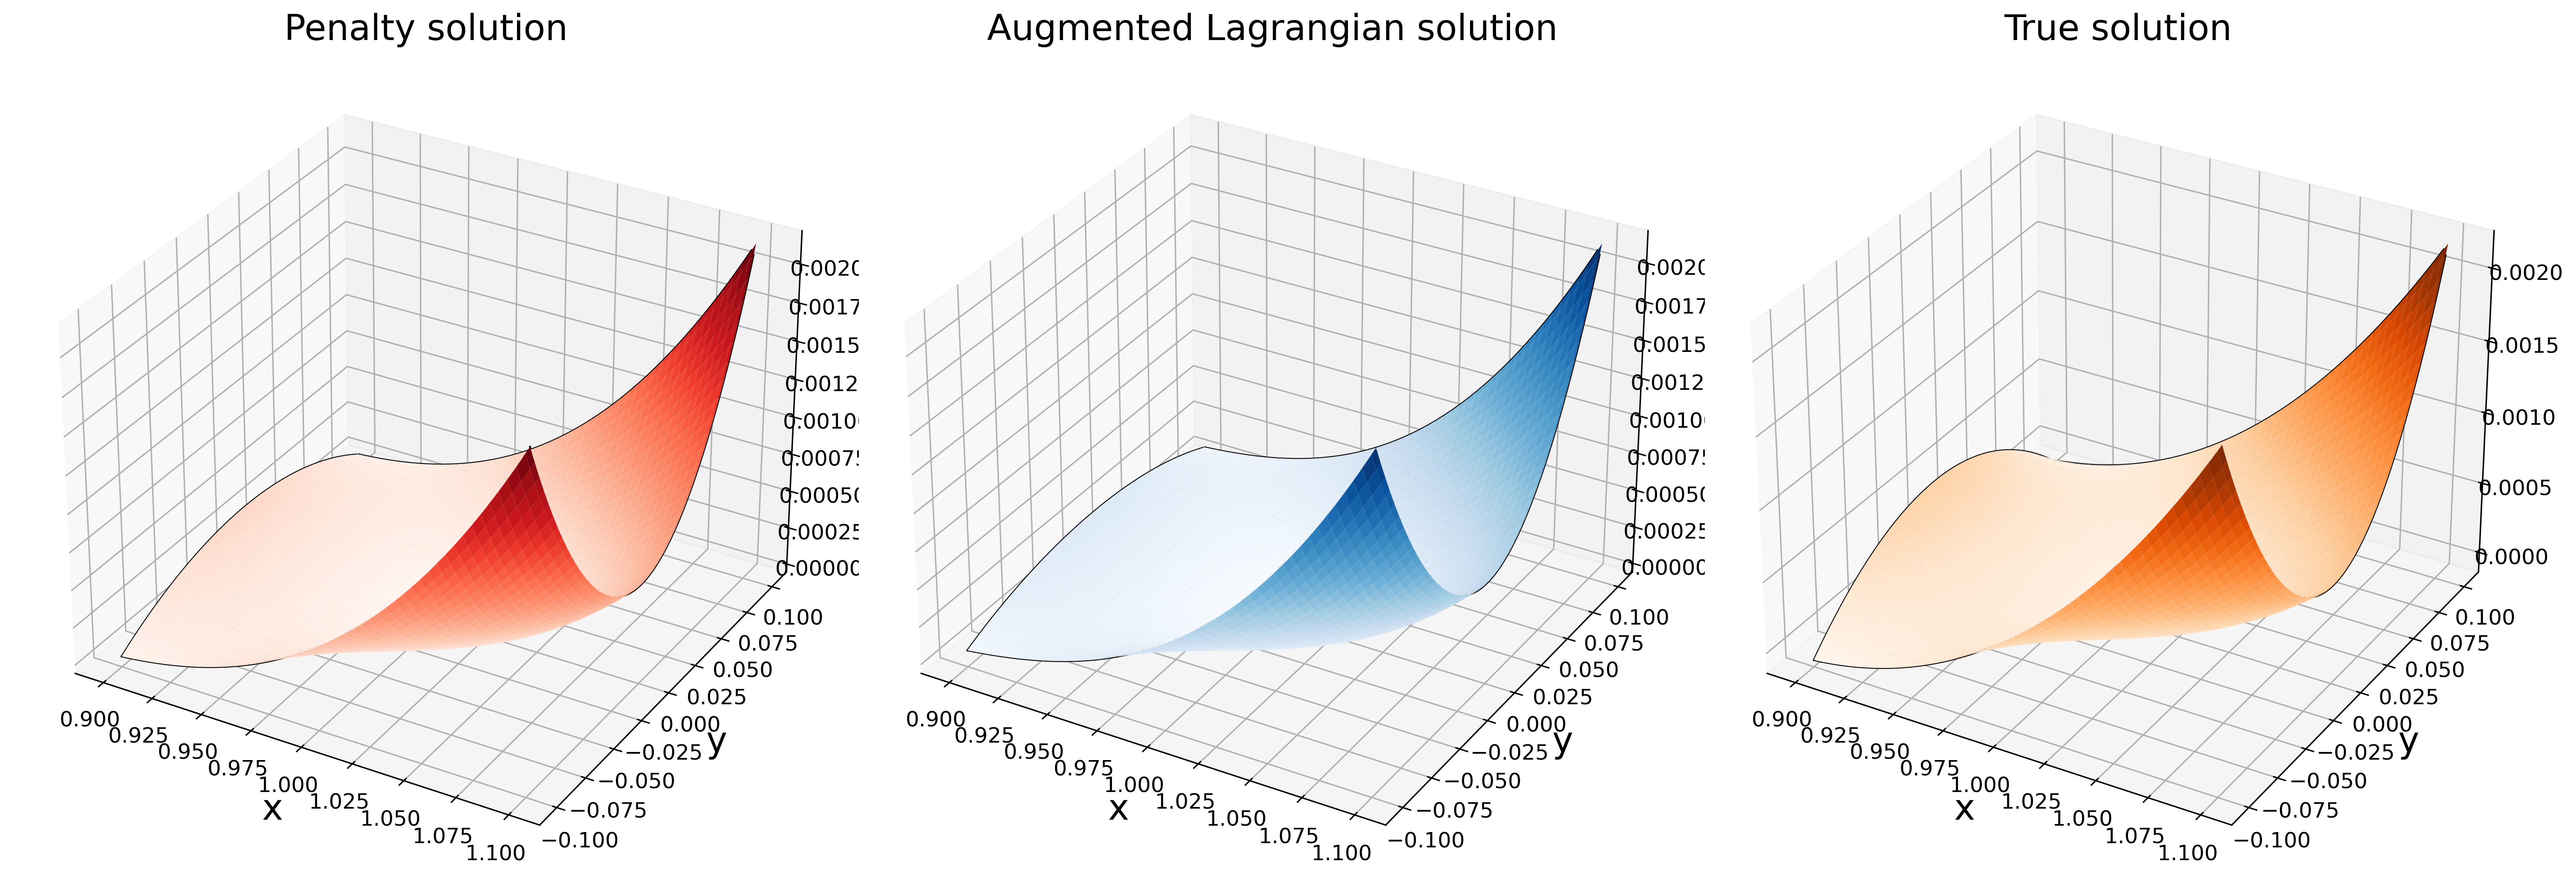
\includegraphics[scale=0.32]{var-ml/plots/var-plots-Grad-Shafranov-surface.png}
    \caption{Solutions to the Grad-Shafranov equation}
    \label{fig:gs-surface--var-ml}
\end{figure}
% For this problem we define the absolute error as,
% \begin{align}
% {\rm absolute\;error}=\sqrt{\frac{\int_{-0.1R}^{0.1R}\int_{0.9R}^{1.1R}(\hat u-u^{\rm true})^2\,dr\,dz}{\int_{-0.1R}^{0.1R}\int_{0.9R}^{1.1R}\,dr\,dz}}   
% \end{align}
We use $E=50000$ and $P=2500$ for this problem which implies that we use $Q=20$ gradient descent steps to solve the subproblems in penalty method (${\rm P}^\infty$) and $Q^A=Q^B=10$ gradient descent steps to solve the subproblems in augmented Lagrangian method (${\rm AL}^\infty_\infty$). Figure~\ref{fig:gs-error--var-ml} shows the various errors and run times for this problem. Both methods produce qualitatively similar error curves. The Lagrange multiplier in this case can be thought of as a function of a single variable since it is a member of $W^{1,2}(\partial\Omega;\mathbb R)$ and $\partial\Omega$ is homeomorphic to a closed curve in $\mathbb R^2$. But for a convenient implementation we represent it as a function of two variables (or on $\Omega$) as seen in table~\ref{tab:network--var-ml}. This does not cause any practical issues since we never encounter the multiplier anywhere expect $\partial \Omega$ during the run time of ${\rm AL}^\infty_\infty$ i.e. we only optimize the multiplier on $\partial\Omega$. According to table~\ref{tab:network--var-ml} the size of the multiplier network $b$ is significantly smaller than the size of the solution network $a$ in this case. These choices reflect the fact that inherently the solution and the multiplier are functions of two and one variables respectively. Even though on a machine, \eqref{eq:seq-uncon-al-net--var-ml} is more expensive to solve than \eqref{eq:seq-uncon-net--var-ml}, since \eqref{eq:xi-update--var-ml} is much cheaper to solve than \eqref{eq:seq-uncon-net--var-ml}, the augmented Lagrangian is ultimately much faster than its counterpart in this case as is seen in figure~\ref{fig:gs-error--var-ml}. 
\begin{figure}[!ht]
    \centering
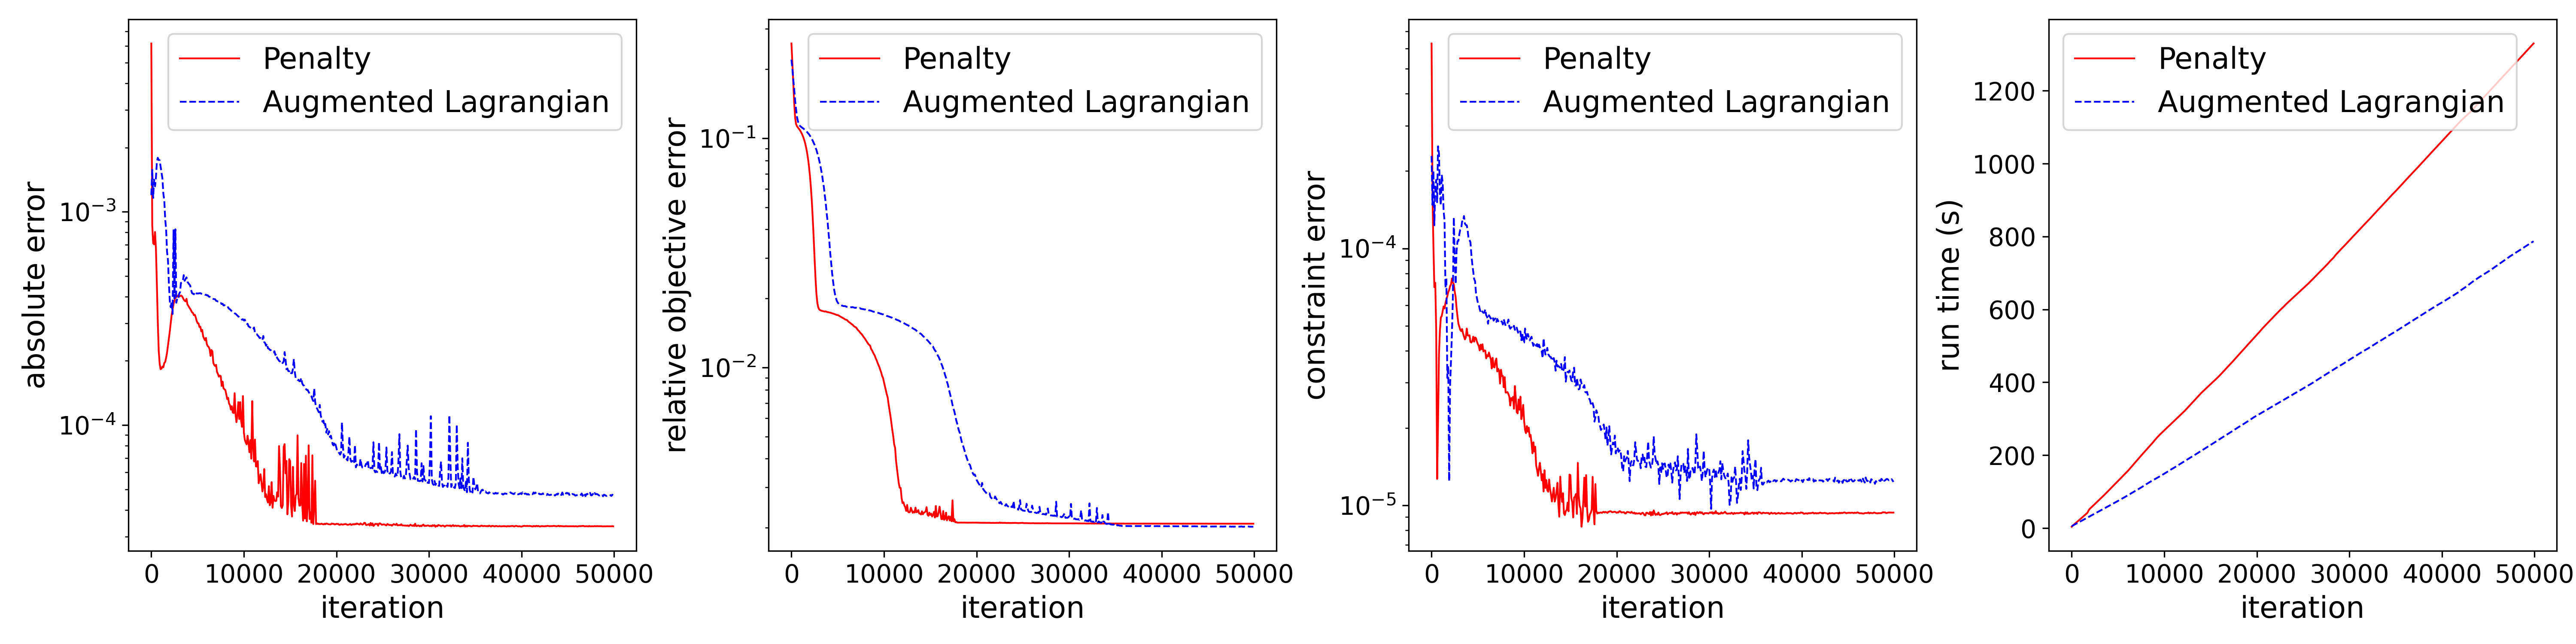
\includegraphics[scale=0.32]{var-ml/plots/var-plots-Grad-Shafranov-error.png}
    \caption{Errors and run times for the Grad-Shafranov problem as functions of gradient descent steps. The errors have been plotted in a semilog fashion. All quantities have been plotted every 100 steps.}
    \label{fig:gs-error--var-ml}
\end{figure}
\subsection{Beltrami fields}
Figure~\ref{fig:bel--var-ml} shows the approximate and true solutions for the Beltrami field problem.
\begin{figure}[!ht]
    \centering
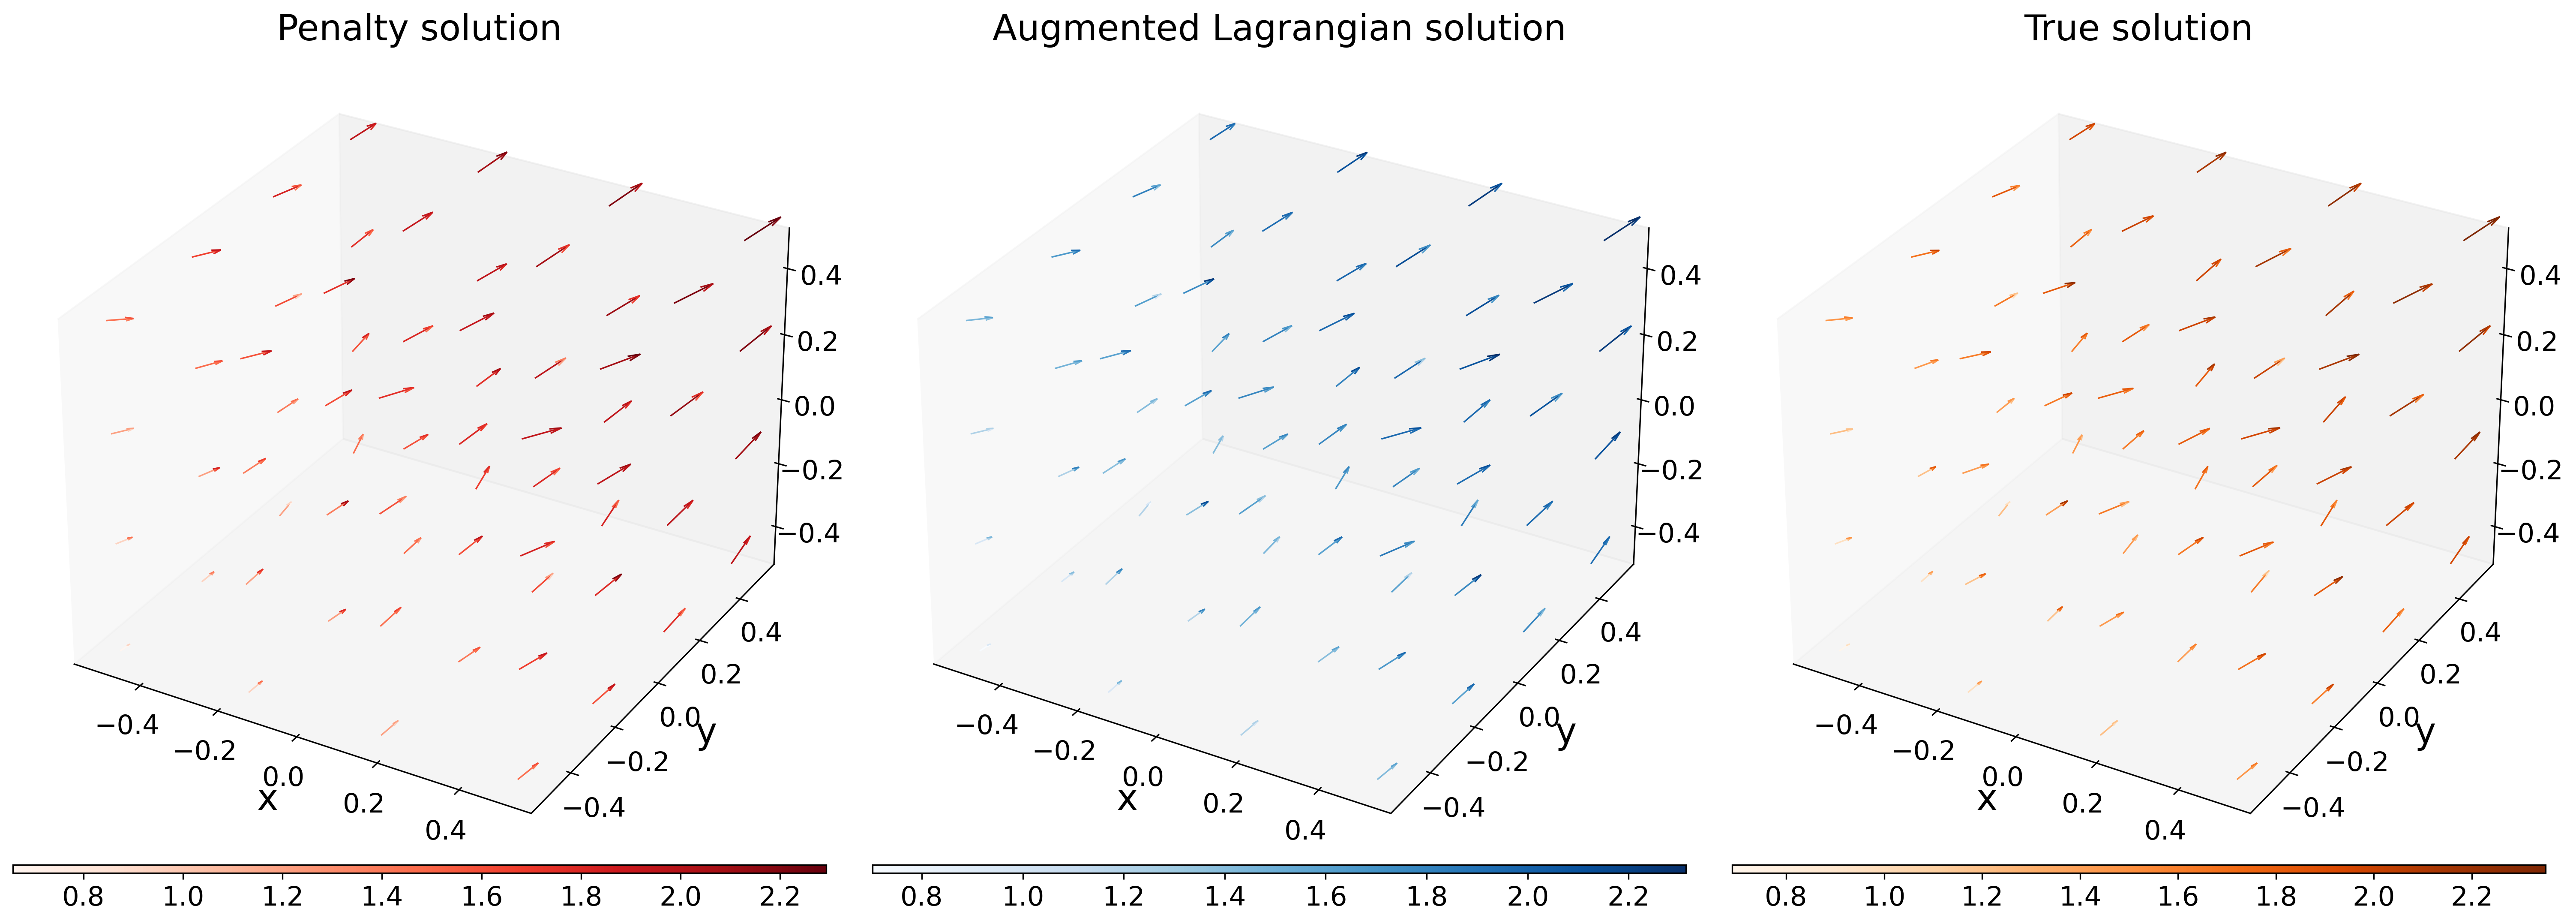
\includegraphics[scale=0.32]{var-ml/plots/var-plots-Beltrami-field.png}
    \caption{Solutions to the Beltrami field problem}
    \label{fig:bel--var-ml}
\end{figure}
 We use $E=50000$ and $P=2500$ for this problem which implies that we use $Q=20$ gradient descent steps to solve the subproblems in penalty method (${\rm P}^\infty$) and $Q^A=Q^B=10$ gradient descent steps to solve the subproblems in augmented Lagrangian method (${\rm AL}^\infty_\infty$). Figure~\ref{fig:bel-error--var-ml} shows the various errors and run times for this problem. In order to enforce Gauss's law we represent the solution magnetic field $\hat u$ as the curl of a vector potential and we represent this vector potential as a neural network $H^{\mathcal A}_{\eta}$, 
 \begin{align}
     \hat u = \nabla\times H^{\mathcal A}_{\eta}
 \end{align}
 This clearly allows many such vector potentials to generate solutions to our problem but we do not concern ourselves with gauge-fixing since we are only interested in the magnetic field $\nabla\times H^{\mathcal A}_{\eta}$ rather than the potential $H^{\mathcal A}_{\eta}$ itself. According to table~\ref{tab:network--var-ml} the vector potential network is much larger than the Lagrange multiplier network in this case. These choices reflect the fact that the solution is a function defined on a volume while the Lagrange multiplier is a function defined on a surface. Just like the previous problem we implement the multiplier as a function of 3 variables while optimizing its values only the boundary $\partial\Omega$ without causing any practical issues. The functional $f$ in this problem requires integration on a 3D volume. To do so we use a Monte-Carlo estimate with only $10^3$ points to maintain a relatively low computational budget. We do achieve qualitatively decent approximations as seen in figure~\ref{fig:bel--var-ml} but our computational parsimony along with the use of the curl operator leading to more floating point operations and errors result in higher absolute and constraint errors compared to the other problems discussed here. The relative computational ease of solving \eqref{eq:xi-update--var-ml} when compared to \eqref{eq:seq-uncon-net--var-ml} results in a faster performance for the augmented Lagrangian algorithm.   
\begin{figure}[!ht]
    \centering
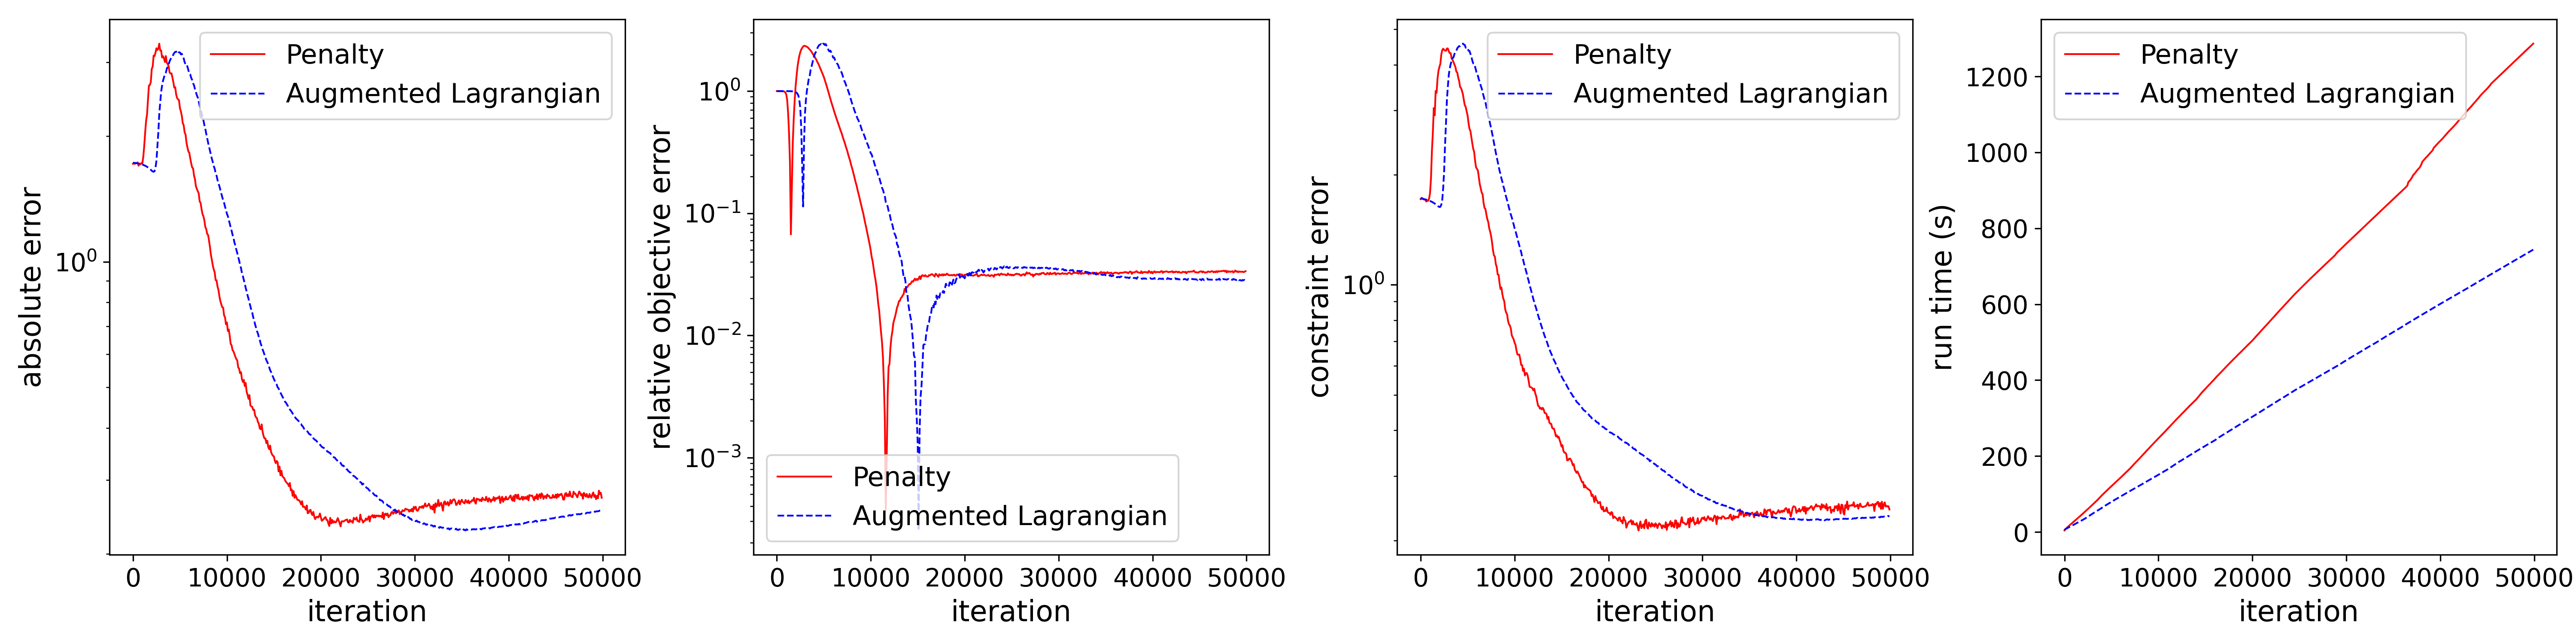
\includegraphics[scale=0.32]{var-ml/plots/var-plots-Beltrami-error.png}
    \caption{Errors and run times for the Beltrami field problem as functions of gradient descent steps. The errors have been plotted in a semilog fashion. All quantities have been plotted every 100 steps.}
    \label{fig:bel-error--var-ml}
\end{figure}